\documentclass[11pt]{article}

\usepackage{exscale}
\usepackage{graphicx}
\usepackage{amsmath}
\usepackage{latexsym}
\usepackage{times,mathptm}
\usepackage{epsfig}

\textwidth 6.5truein          
\textheight 9.0truein
\oddsidemargin 0.0in
\topmargin -0.6in

\parindent 0pt          
\parskip 5pt
\def\baselinestretch{1.1}

\begin{document}

\begin{LARGE}
\centerline {\bf CSci 423 Homework 1}
\end{LARGE}
\vskip 0.25cm

\centerline{Due: 1:00 pm, Wednesday, 9/12}
\centerline{Eric Shih}


\begin{enumerate}

\item (5 points) Prove by induction that for all integers $n \ge 4$ the inequality $2^n < n!$ holds.
\begin{description}
 \item Basis Step: $2^n<n!$ when $n = 4$ \\
  $\implies$ $16 ? 24$ \\
 $\implies$ $2^4 ? 4 \cdot 3 \cdot 2 \cdot 1$ \\
 $\implies$ $2^4 ? 4!$ \\
The basis step is confirmed

 \item Inductive Hypothesis: \\
  $\forall k$ assume $2^k < k!$ for some $k \leq n$ where $k > 4$

 \item Inductive Step: \\
  We wish to prove $n = k+1$ such that $2^{k+1} < (k+1)!$ \\
  $\implies 2^k \cdot 2 < k+1 \cdot k!$ \\
  Since $k>2$ as shown before, we can assume that by the inductive hypothesis that $2^{k+1} < (k+1)!$

\end{description}

\item (5 points) Prove by contradiction that $2 - \sqrt{2}$ is not a rational number. \\
\begin{description}
 \item First, let us assume that an irrational number plus a rational number makes a rational number and make this lead to a contradiction.\\
      If a is rational, b is irrational, and c is rational, we will try to prove that $a + b = c$ is rational. If this is true, $a = x/y$
      and $c = e/f$ for integers x, y, e, and f. So:
  \item $a + b = c$ \\
	$\implies x/y + b = e/f$ \\
	$\implies b = e/f - x/y$ \\
	$\implies b = ey/(fy) - xf/(fy)$ \\
	$\implies b = (ey - xf)/(fy)$
  \item Since the RHS is rational, so is b. But we said that b is irrational! This leads to a contradiction and so the sum must be irrational.
\end{description}



\begin{description}
\item We know, from the proof cited before, that any sum of a rational and irrational number is irrational, so we will first focus on  $\sqrt{2}$.
To prove by contradiction we first assume $\sqrt{2}$ is a rational number.
\item $\exists$ int a, b with $gcd(a,b)=1$, such that $\sqrt{2} = \frac{a}{b}$\\
 $\implies$ $2=\frac{a^2}{b^2}$ \\
 We then find the greatest common denominator (gcd) of a and b. \\
 $\exists k$ $a=2k \implies (2k)^2=2b^2$\\
 $\exists l$ $b=2l$
\item From this, we deduce that the $gcd(a,b) \geq2$, which contradicts the fact that $gcd(a,b)=1$, and proves $\sqrt{2}$
 irrational. Therefore if $\sqrt{2}$ is irrational, $2 - \sqrt{2}$ is irrational by the properties of irrational 
 numbers.
\end{description}

\item (5 points) Find the error in the following proof that all horses are the same color. \\
There is an incorrect claim when $H_1$ is presented as having $k$ horses where $h=k$. The inductive step is not applies to the base case,
therefore no way to know what color of the set of horses is. The entire proof relies on this property, and since it cannot be verified, the rest of the proof is false.

\item (5 points for each question) Give state diagrams of DFAs recognizing the followiing languages. In all parts the alphabet is $\{0,1\}$.

\begin{enumerate}

\item[a.] $\{w|w$ begins with a 1 and ends with a 0$\}$
\begin{center}
  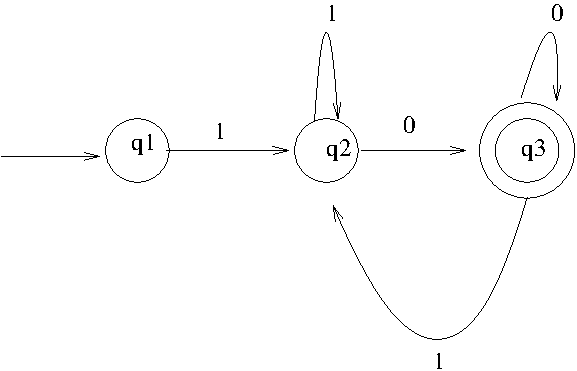
\includegraphics[scale=.4] {fig1.pdf}
\end{center}

\item[e.] $\{w|w$ starts with 0 and has odd length, or starts with 1 and has even length$\}$
\begin{center}
  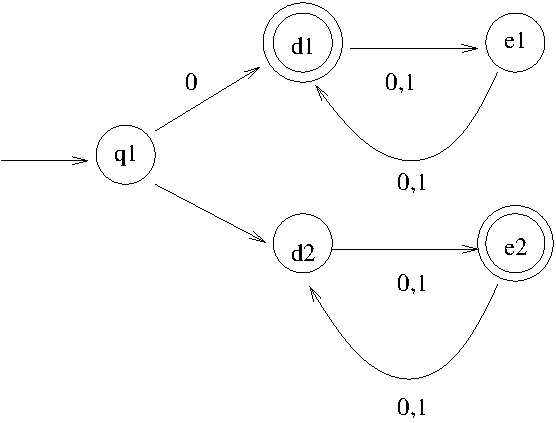
\includegraphics[scale=.4] {fig2.pdf} \\
  d = odd, e = even
\end{center}

\item[i.] $\{w|$ every odd position of $w$ is a 1$\}$
\begin{center}
  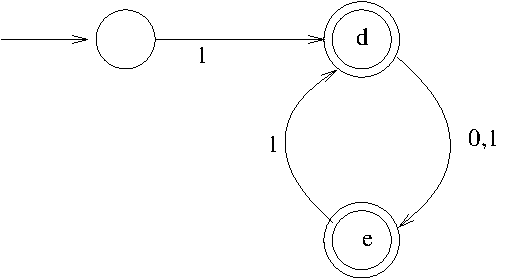
\includegraphics[scale=.4] {fig3.pdf} \\
  d = odd, e = even
\end{center}

\item[n.] All strings except the empty string
\begin{center}
  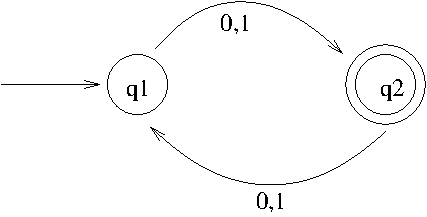
\includegraphics[scale=.4] {fig4.pdf}
\end{center}
\end{enumerate}

\item (5 points) Give the state diagram of a DFA that recognizes (accepts) the set of strings such that in each string the number of 0s is divisible by 5 and the number of 1s is divisible by 3.
\begin{center}
  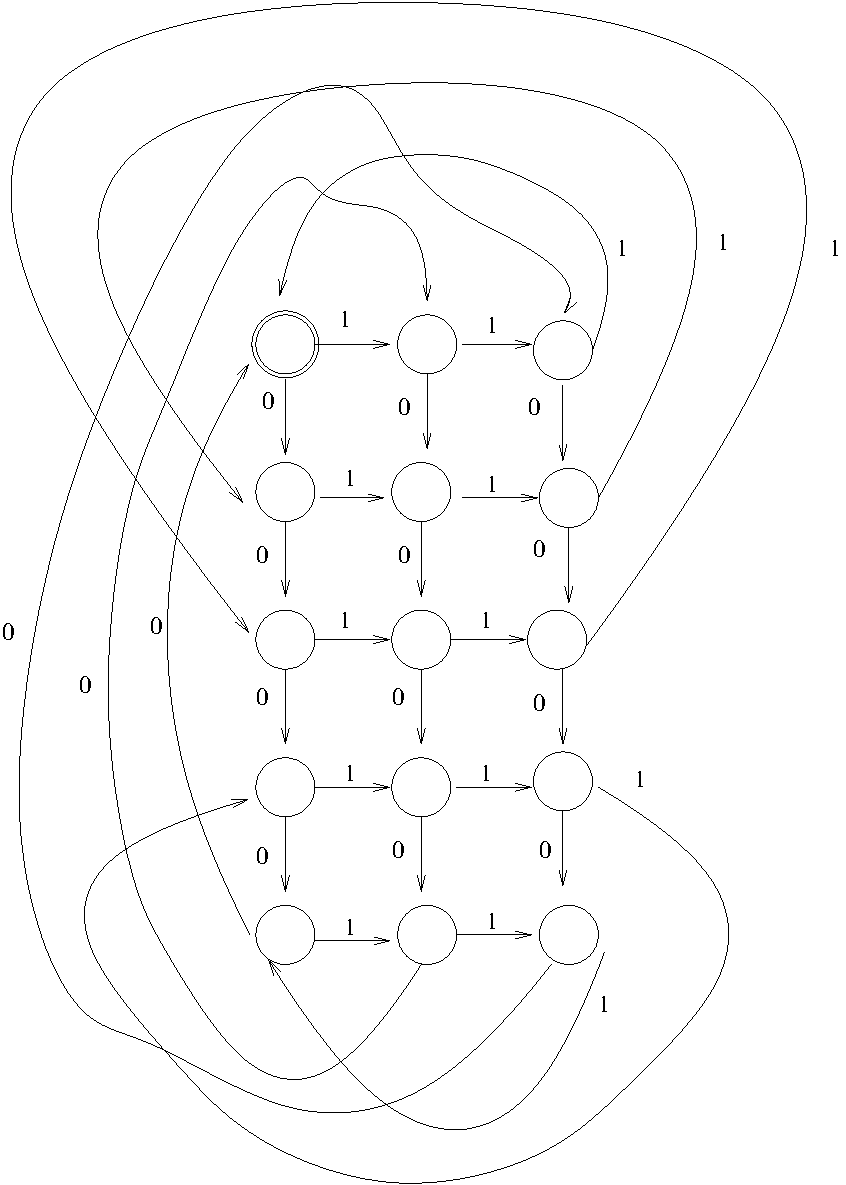
\includegraphics[scale=.4] {fig5.pdf}
\end{center}
\end{enumerate}

\end{document}